\chapter{Black-Scholes Model}
\label{ch:BS}

\section{Black-Scholes Model}
Suppose that stock price $S$ follows a geometric Brownian motion

\begin{equation}
dS = \mu Sdt + \sigma SdW
\label{eq:bs_gbm}
\end{equation}
we are going to derive a partial differential equation (PDE) for the price of a derivative based on such a stock.

The model proposed by Black and Scholes relies on the following set of additional assumptions (besides the geometric Brownian motion):
\begin{itemize}
\tightlist 
\item constant risk-less interest rate $r$;
\item no transaction costs;
\item it is possible to buy/sell any (also fractional) number of stocks; similarly with the cash;
\item no restrictions on short selling;
\item option is of European type.
\end{itemize}

After the derivation of the model equation we will determine the explicit solution for European call and put options.

\subsection{Merton Derivation}
In this Section we are going to provide the steps followed by Merton to derive the Black-Scholes PDE.

Firstly, let's consider the case of a non-dividend paying stock. Imagine a portfolio consisting of options, stocks and cash with the properties that at each time $t$ the portfolio has zero value and it is \emph{self-financing}, which means that if there is no exogenous infusion or withdrawal of money, the purchase of a new asset must be financed by the sale of an old one. Let be 
\begin{itemize}
\item $Q_S$, the number of stocks, each of them with value $S$;
\item $Q_V$, number of options, each of them with value $V$;
\item $B$, cash on the account, which is continuously compounded using the risk-free rate $r$.
\end{itemize}
The required properties can be formulated mathematically as
\begin{equation}
\begin{cases}
SQ_S+VQ_V+B=0 \\
SdQ_S + V dQ_V +\delta B = 0 \\
dB = rBdt+\delta B
\end{cases}
\label{eq:bs_properties}
\end{equation}
Differentiating the first of Eq.~\ref{eq:bs_properties}
\begin{equation}
\begin{split}
&d(SQ_S + VQ_V +B) = d(SQ_S + VQ_V) + \overbrace{dB}^{rBdt+\delta B} = 0 \\
& \overbrace{SdQ_s + VdQ_V +\delta B}^{=0} + Q_S dS + Q_V dV + rBdt = 0 \\
& Q_SdS+Q_VdV \overbrace{-r(SQ_S + VQ_V)}^{rB}dt=0\\
\end{split} 
\end{equation}
Dividing by $Q_V$ and setting $\Delta = -\frac{Q_S}{Q_V}$
\begin{equation}
dV -rVdt-\Delta (dS - rSdt)=0
\end{equation}
$dS$ can be determined from Eq.~\ref{eq:bs_gbm}, while $dV$ applying It$\hat{o}$'s lemma. Then we choose $\Delta$ (i.e. the ratio between the number of stocks and options) so that it eliminates the randomness (i.e. the coefficient at $dW$ is zero).
  
\begin{equation}
dV = \left(\cfrac{\partial V}{\partial t} + \mu S  \cfrac{\partial V}{\partial S} + \cfrac{1}{2} \sigma^2 S^2  \cfrac{\partial^2 V}{\partial S^2} \right) dt + \sigma S \cfrac{\partial V}{\partial S} dW
\end{equation} 
Therefore:
\begin{equation}
dP =  \left(\cfrac{\partial V}{\partial t} + \mu S  \cfrac{\partial V}{\partial S} + \cfrac{1}{2} \sigma^2 S^2  \cfrac{\partial^2 V}{\partial S^2} + \delta \mu S\right) dt + \left(\sigma S  \cfrac{\partial V}{\partial S} + \delta \sigma S \right)dW
\end{equation}
We eliminate the randomness
\begin{equation}
\delta = -\cfrac{\partial V}{\partial S}
\end{equation}

\begin{equation}
\cfrac{\partial V}{\partial t} + \cfrac{1}{2} \sigma^2 S^2 \cfrac{\partial^2 V}{\partial S^2}+ rS \cfrac{\partial V}{\partial S} - rV = 0
\end{equation}

\section{Solutions of Black-Scholes PDE}
Now we need to find a solution $V(S, t)$ to the partial differential equation which holds for $S >0$, $t \in [0, T)$.

So far we have not used the fact that we consider an option (in general the PDE holds for any derivative that pays a payoff at time $T$ depending on the stock price at this time).
Clearly the type of derivative determines the terminal condition at time $T$, so in general $V(S, T)$ = payoff of the derivative.

\subsection{Simple Solutions}
How to price the derivatives with the following payoffs:
\begin{itemize}
\tightlist
\item $V(S, T) = S$, it is in fact a stock so $V(S, t) = S$
\item $V(S, T) = E$ with a certainty we obtain the cash $E$ ($V(S, t) = Ee^{-r(T-t)}$)
\end{itemize}
by substitution into the PDE it is possible to check that they are indeed solutions.
%EXERCISES:
%Find the price of a derivative with payoff
%$V(S, T) =S^n$,where $n\in N$.

%HINT: Look for the solution in the form
%$V(S, t) =A(t)S^n$

%Find all solutions to the Black-Scholes PDE, which are independent of time, i.e., for which
%$V(S, t) = V(S)$

\subsection{Binary Options}
Let us consider a binary option, which pays \$1 if the stock price is higher than $K$ at expiration time, otherwise its payoff is zero.
In this case
\begin{equation}
V(S, T) = 
\begin{cases}
  1, \quad\textrm{if }S > K\\
  0, \quad\textrm{otherwise}	
\end{cases}
\end{equation}

This partial differential equation (PDE) can be solved directly with numerical methods. But then some tricky stability issues must be tackled. Here we prefer applying variable transformations as much as possible in order to obtain a simpler form (i.e. the goal is to re-formulate Black-Scholes PDE into a heat equation).

The first step is to apply the transformation $x = \textrm{ln}(S/K)$ and a new function $Z(x, \tau) = V (Ee^x, T -\tau)$. 
The PDE for $Z(x, \tau)$ becomes:
\begin{equation}
\begin{gathered}
\cfrac{\partial Z}{\partial \tau}-\cfrac{1}{2}\sigma^2 \cfrac{\partial^2 Z}{\partial x^2}+\left(\cfrac{\sigma^2}{2}-r\right)  \cfrac{\partial Z}{\partial x} + rZ = 0\\ \\
Z(x, 0) =V(Ee^x, T)
\end{gathered}
\end{equation}
Then consider the new function $u(x,\tau)=e^{\alpha x + \beta\tau}Z(x,\tau)$ where the constants $\alpha, \beta \in \mathbb{R}$ are chosen so that the PDE for $u$ is the heat equation.

The corresponding PDE for $u$ is
\begin{equation}
\begin{gathered}
\cfrac{\partial u}{\partial \tau} -\cfrac{\sigma^2}{2} \cfrac{\partial^2 u}{\partial x^2}+A\cfrac{\partial u}{\partial x} + Bu = 0\\ \\
u(x,0)=e^{\alpha x}Z(x,0)=e^{\alpha x}V(Ke^x, T)
\end{gathered}
\end{equation}
where
\begin{equation}
\begin{cases}
A=\alpha\sigma^2 + \cfrac{\sigma^2}{2}-r\\
B=(1+\alpha)r-\beta-\cfrac{\alpha^2\sigma^2+\alpha\sigma^2}{2}
\end{cases}
\end{equation}
In order to have $A=B=0$ to get the heat equation we set
\begin{equation}
\begin{cases}
\alpha=\cfrac{r}{\sigma^2}-\cfrac{1}{2}\\
\beta=\cfrac{r}{2}+\cfrac{\sigma^2}{8}+\cfrac{r^2}{2\sigma^2}
\end{cases}
\end{equation}
The solution $u(x,\tau)$ of the resulting PDE is given by the \emph{Green formula}
\begin{equation}
u(x, \tau)=\cfrac{1}{\sqrt{2\sigma^2\pi\tau}}\int^{+\infty}_{-\infty}e^{-\frac{(x-s)^2}{2\sigma^2\tau}}u(s,0)ds
\end{equation}

After evaluating the integral it is possible to find the original solution $V(S,t)$ performing backward substitutions

\begin{equation}
V(S, t) = e^{-r(T-t)}N(d_2)
\end{equation}
where $d_2=\frac{\textrm{log}(\frac{S}{K}+\left(r-\frac{\sigma^2}{2}\right)(T-t)}{\sigma\sqrt{T-t}}$.

\subsection{Call Options}
In this case
\begin{equation}
V(S,T)=\textrm{max}(0,S-K)=
\begin{cases}
S-K,\quad \textrm{if}~S>K\\
0, \quad\textrm{otherwise}
\end{cases}
\end{equation}

The steps are similar to the previous example (i.e. same sequence of transformations, initial conditions for the heat equation):
\begin{equation}
u(x,0)=
\begin{cases}
e^{\alpha x}(S-K),\quad \textrm{if}~x>0\\
0, \quad\textrm{otherwise}
\end{cases}
\end{equation}
and similar evaluation of the integral. Finally the option price
\begin{equation}
V(S,t) = SN(d_1)-Ke^{-r(T-t)}N(d_2)
\end{equation}
where $N$ is the distribution function of a normalized normal distribution and  $d_1=\frac{\textrm{log}(\frac{S}{K}+\left(r+\frac{\sigma^2}{2}\right)(T-t)}{\sigma\sqrt{T-t}}$, $d_2=d_1-\sigma\sqrt{T-t}$.

Figure~\ref{fig:call_option} shows the option price as a function of the stock price for various values of $t$.

\begin{figure}[htb]
  \centering
  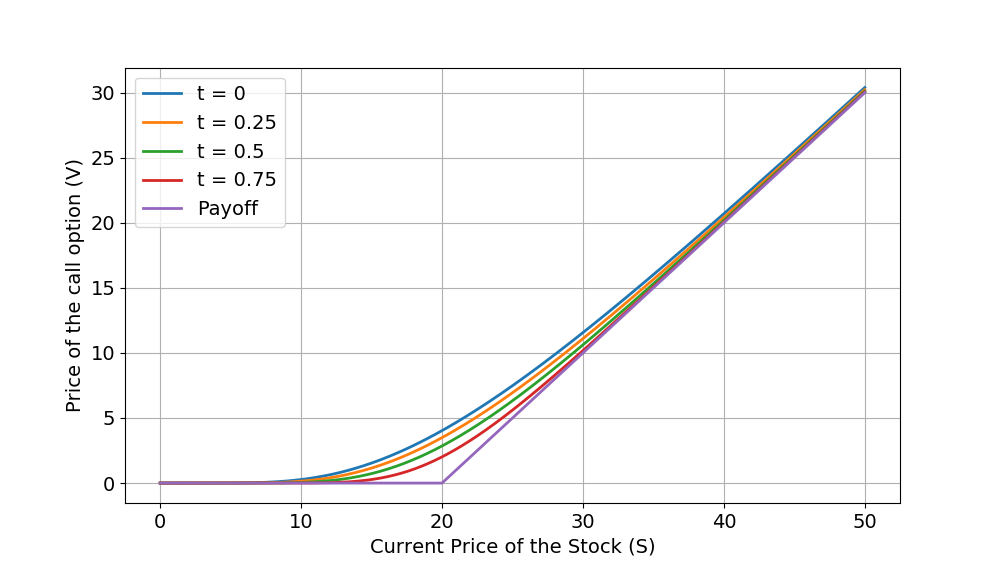
\includegraphics[width=0.9\textwidth]{figures/call_option_price}
  \caption{Option price as a function of the underlying price for various values of $t$.}
  \label{fig:call_option}
\end{figure}

\section{Asian Options}
\label{sec:asian_option}

An Asian option is a special option where the payoff is determined by \emph{the average underlying price over some preset-set period of time}; 
Asian options are thus one of the basic forms of exotic options. 

One advantage of Asian options is that these reduce the risk of market manipulation of the underlying instrument at maturity.
Because of the averaging feature, Asian options reduce the volatility inherent in the option; therefore, Asian options are typically cheaper than European or American options. 

There are numerous permutations of Asian option; the most basic are listed below:
\begin{itemize}
\item \textbf{Fixed strike} Asian call payout
$C(T)={\text{max}}\left(A(0,T)-K,0\right),$
where $A$ denotes the average price for the period $[0, T]$, and $K$ is the strike price. 
The equivalent put option is given by
$P(T)={\text{max}}\left(K-A(0,T),0\right)$.

\item The \textbf{floating strike} Asian call option has the payout
$C(T)={\text{max}}\left(S(T)-kA(0,T),0\right),$
where $S(T)$ is the price at maturity and $k$ is a weighting, usually 1 so often omitted from descriptions.
The equivalent put option payoff is given by
$P(T)={\text{max}}\left(kA(0,T)-S(T),0\right)$.
\end{itemize}

The average $A$ may be obtained in many ways. Conventionally, this means an arithmetic average. In the continuous case, this is obtained by
$A(0,T)={\frac  {1}{T}}\int _{{0}}^{{T}}S(t)dt$.
For the case of discrete monitoring (with monitoring at the times 
$0=t_{0},t_{1},t_{2},\dots ,t_{n}=T$ we have the average given by
${\displaystyle A(0,T)={\frac {1}{n}}\sum _{i=1}^{n}S(t_{i}).}$

There also exist Asian options with geometric average; in the continuous case, this is given by
$A(0,T)=\exp \left({\frac  {1}{T}}\int _{{0}}^{{T}}\ln(S(t))dt\right)$.

\subsection{Pricing of Asian options}
We are able to derive a closed-form solution only for the geometric Asian option.
This is given by 
\begin{equation}
\begin{aligned}
C_A&=S_{0}e^{(b-r)T}\Phi (d_{1})-Ke^{-rT}\Phi (d_{2})\\
P_A&=Ke^{-rT}\Phi (-d_{2})-S_{0}e^{(b-r)T}\Phi (-d_{1})
\end{aligned}
\end{equation}
where 
\begin{equation}
\begin{aligned}
b&={1 \over {2}}\left(r-{1 \over {2}}\sigma _A^{2}\right)\\
\sigma _A&={\sigma  \over {\sqrt {3}}} \\
d_1&={\log {S_0 \over {K}}+\left(b+{1 \over {2}}\sigma _A^2\right)T \over {\sigma_A{\sqrt {T}}}},\;d_{2}=d_1-\sigma_A{\sqrt {T}}
\end{aligned}
\end{equation}

The arithmetic average type instead needs to be estimated with Monte Carlo techniques.

\subsection{Asian Option Pricing with Monte Carlo}

Every time a Monte Carlo simulation is run, we get an estimate of the quantity we are trying to calculate. It is desirable to quantify how precise our estimate is through the "standard error" (i.e. confidence interval).

As we have seen above an obvious way to make our estimate more precise is to increase the number $N$ of simulations (e.g. random price paths) considered. However this can be computationally expensive therefore different methods have been developed, namely \emph{variance reduction techniques}.

\subsubsection{Antithetic Method}
Let $\theta$ be estimated through $Y$, that is $\theta=\mathbb{E}[Y]$. Let $Y_1$ and $Y_2$ be two samples of $Y$, so the estimate is $\hat{\theta}=\frac{Y_1+Y_2}{2}$. The variance of the estimate is 
\begin{equation*}
\text{Var}(\hat{\theta}) = \frac{\text{Var}(Y_1)+\text{Var}(Y_2)+2\text{Cov}(Y_1,Y_2)}{4}
\end{equation*}

If $Y_1$ and $Y_2$ are i.i.d. $\text{Var}(\hat{\theta})=\frac{\text{Var}(Y)}{2}$, and if $\text{Cov}(Y_1, Y_2)<0$ the variance is reduced even more. In the extreme case where $\rho=-1$, the variance is reduced to the maximum allowed by this technique. 

Since the path of the stock is defined as a geometric Brownian motion with random normal shocks, $Y_1$ can be a set of normal random numbers and $Y_2 = -Y_1$. Hence the final payoff is given by the average between two sets of payoffs computed respectively with $Y_1$ and $Y_2$ which by construction are \emph{perfectly anti-correlated}. 

\subsubsection{Control Variate Variance Reduction Method}

Say desired simulation quantity is $\mathbb{E}[X]$, and there is another known random variable $Y$ with known analytical expectation $\mu_Y = \mathbb{E}[Y]$. For any constant $c$ one can see that $Z = X + c\cdot(Y -\mu_Y)$ is an unbiased estimator of $X$, by linearity of expectation. Also it can be shown that $\text{Var}(Z) = \text{Var}(X) + 2c\cdot \text{Var}(Y) + 2c\cdot\text{Cov}(X; Y)$ is minimized when $c = -\frac{\text{Cov}(X;Y)^2}{\text{Var}(Y)}$. 
$Y$ is called a \textbf{control variate} of $X$. 

To reduce variance, $Y$ can be chosen as much correlated as possible with $X$. In practice, we can select a $Y$ which is approximately equal to $X$, easy to simulate and whose expectation is known. 

In our case given that $X$ is the payoff of an Asian Option with Arithmetic average, these requirements are satisfied perfectly when we take $Y$ to be the Asian Option payoff with Geometric average (a closed form solution for its price is known).

In practice we are going to simulate a set of paths for the underlying and compute $Z$ from  $X$, $Y$ and $\mu_Y$.

\begin{finmarkets}
The following class \texttt{AsianOption} implements all the methods described above besides the analytical pricing formula of the Geometric average Asian option.
\end{finmarkets}

\pythoncode{code/options_1.py}

\subsubsection{An Example}
We are going to consider an Asian Option (fixed strike) with the following properties
\begin{ipython}
S0 = 100 #underlying price
K = 100 # strike
tau = 1 # time to maturity (years)
sigma = 0.2 # volatility
r = 0.05 # constant risk-free rate
\end{ipython}
and compare the results from the different Monte Carlo techniques.

The baseline result is represented by a "naive" Monte Carlo simulation where various underlying price paths are generated with the Euler scheme. The option price is determined as the mean of the discounted payoffs corresponding to each simulation
\begin{equation*}
C = \frac{1}{N}\sum_{i=1}^{N} e^{-r\tau}\max(0, A_i(0, \tau)-K)
\end{equation*}

Baseline results are compared to analogous simulations performed with antithetic and control variate techniques.
Figures~\ref{fig:asian_mc_results} shows the comparison of prices and uncertainties as a function of $N$ and $K=100$.
In general the larger the number of simulations, the more accurate the estimate.
One can see also that with control variates, the option value is almost constant, whereas the naive implementation tends to jump around before converging.

%\begin{table}[h]
%\begin{center}
%\begin{tabular}{l|c|c|c|c|c} 
%  \hline
%  & 80 & 90 & 100 & 110 & 120 \\
%  \hline
%  100 & 20.845 & 12.005 & 5.250 & 1.549 & 0.386 \\ 
%  \hline
%  1000 & 21.403 & 12.455 & 5.670 & 1.949 & 0.531 \\ 
%  \hline
%  10000 & 21.313 & 12.434 & 5.621 & 1.915 &  0.496 \\ 
%  \hline
%  100000 & 21.461 & 12.553 & 5.721 & 1.967 &  0.519 \\ 
%  \hline
%  1000000 & 21.489 & 12.591 & 5.754 & 1.981 &  0.522 \\ 
%\end{tabular}
%\end{center}
%\end{table}
%
%
%\begin{table}[h]
%\begin{center}
%\begin{tabular}{l|c|c|c|c|c} 
%  \hline
%  & 80 & 90 & 100 & 110 & 120 \\
%  \hline
%  100 & 1.0870 & 0.9900 & 0.7425 & 0.4388 & 0.2595 \\ 
%  \hline
%  1000 & 0.3543 & 0.3292 & 0.2524 & 0.1560 & 0.0807 \\ 
%  \hline
%  10000 & 0.1118 & 0.1027 & 0.0783 & 0.0473 &  0.0231 \\ 
%  \hline
%  100000 & 0.0335 & 0.0328 & 0.0251 & 0.0153 &  0.0077 \\ 
%  \hline
%  1000000 & 0.0113 & 0.0104 & 0.0080 & 0.0049 &  0.0025 \\ 
%\end{tabular}
%\end{center}
%\end{table}
%
%
%\begin{table}[h]
%\begin{center}
%\begin{tabular}{l|c|c|c|c|c} 
%  \hline
%  & 80 & 90 & 100 & 110 & 120 \\
%  \hline
%  100 & 20.845 & 12.005 & 5.250 & 1.549 & 0.386 \\ 
%  \hline
%  1000 & 21.403 & 12.455 & 5.670 & 1.949 & 0.531 \\ 
%  \hline
%  10000 & 21.313 & 12.434 & 5.621 & 1.915 &  0.496 \\ 
%  \hline
%  100000 & 21.461 & 12.553 & 5.721 & 1.967 &  0.519 \\ 
%  \hline
%  1000000 & 21.489 & 12.591 & 5.754 & 1.981 &  0.522 \\ 
%\end{tabular}
%\end{center}
%\end{table}
%
%
%\begin{table}[h]
%\begin{center}
%\begin{tabular}{l|c|c|c|c|c} 
%  \hline
%  & 80 & 90 & 100 & 110 & 120 \\
%  \hline
%  100 & 1.0870 & 0.9900 & 0.7425 & 0.4388 & 0.2595 \\ 
%  \hline
%  1000 & 0.3543 & 0.3292 & 0.2524 & 0.1560 & 0.0807 \\ 
%  \hline
%  10000 & 0.1118 & 0.1027 & 0.0783 & 0.0473 &  0.0231 \\ 
%  \hline
%  100000 & 0.0335 & 0.0328 & 0.0251 & 0.0153 &  0.0077 \\ 
%  \hline
%  1000000 & 0.0113 & 0.0104 & 0.0080 & 0.0049 &  0.0025 \\ 
%\end{tabular}
%\end{center}
%\end{table}
%
%\begin{table}[h]
%\begin{center}
%\begin{tabular}{l|c|c|c|c|c} 
%  \hline
%  & 80 & 90 & 100 & 110 & 120 \\
%  \hline
%  100 & 21.385 & 12.377 & 5.577 & 1.761 & 0.428 \\ 
%  \hline
%  1000 & 21.483 & 12.561 & 5.723 & 1.939 & 0.508 \\ 
%  \hline
%  10000 & 21.472 & 12.576 & 5.720 & 1.967 &  0.517 \\ 
%  \hline
%  100000 & 21.476 & 12.572 & 5.731 & 1.963 &  0.512 \\ 
%  \hline
%  1000000 & 21.483 & 12.585 & 5.749 & 1.979 &  0.521 \\ 
%\end{tabular}
%\end{center}
%\end{table}
%
%\begin{table}[h]
%\begin{center}
%\begin{tabular}{l|c|c|c|c|c} 
%  \hline
%  & 80 & 90 & 100 & 110 & 120 \\
%  \hline
%  100 & 0.1299 & 0.3639 & 0.2373 & 0.2925 & 0.1592 \\ 
%  \hline
%  1000 & 0.0464 & 0.1233 & 0.0817 & 0.0999 & 0.0555 \\ 
%  \hline
%  10000 & 0.0135 & 0.0390 & 0.0253 & 0.0312 &  0.0166 \\ 
%  \hline
%  100000 & 0.0043 & 0.0123 & 0.0080 & 0.0099 &  0.0053 \\ 
%  \hline
%  1000000 & 0.0014 & 0.0039 & 0.0026 & 0.0031 &  0.0017 \\ 
%\end{tabular}
%\end{center}
%\end{table}
%
%\begin{table}[h]
%\begin{center}
%\begin{tabular}{l|c|c|c|c|c} 
%  \hline
%  & 80 & 90 & 100 & 110 & 120 \\
%  \hline
%  100 & 21.460 & 12.576 & 5.761 & 1.998 & 0.509 \\ 
%  \hline
%  1000 & 21.494 & 12.598 & 5.762 & 1.993 & 0.536 \\ 
%  \hline
%  10000 & 21.488 & 12.590 & 5.758 & 1.986 &  0.527 \\ 
%  \hline
%  100000 & 21.490 & 12.593 & 5.758 & 1.986 &  0.525 \\ 
%  \hline
%  1000000 & 21.490 & 12.593 & 5.758 & 1.986 &  0.525 \\ 
%\end{tabular}
%\end{center}
%\end{table}
%
%\begin{table}[h]
%\begin{center}
%\begin{tabular}{l|c|c|c|c|c} 
%  \hline
%  & 80 & 90 & 100 & 110 & 120 \\
%  \hline
%  100 & 0.0249 & 0.0221 & 0.0190 & 0.0146 & 0.0131 \\ 
%  \hline
%  1000 & 0.0101 & 0.0088 & 0.0074 & 0.0065 & 0.0063 \\ 
%  \hline
%  10000 & 0.0029 & 0.0025 & 0.0021 & 0.0019 &  0.0017 \\ 
%  \hline
%  100000 & 0.0009 & 0.0008 & 0.0007 & 0.0006 &  0.0006 \\ 
%  \hline
%  1000000 & 0.0003 & 0.0003 & 0.0002 & 0.0002 &  0.0002 \\ 
%\end{tabular}
%\end{center}
%\end{table}

\begin{figure}{h}
  \begin{center}
    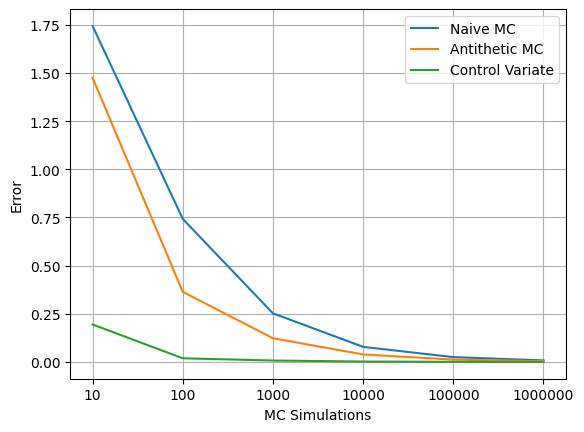
\includegraphics[width=0.4\linewidth]{figures/asian_option_price}
    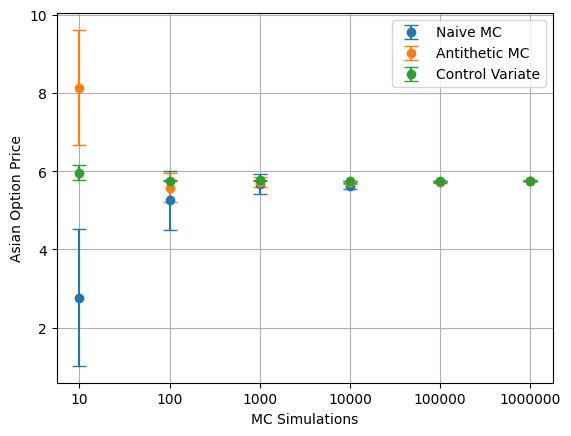
\includegraphics[width=0.4\linewidth]{figures/asian_option_error}
  \end{center}
  \caption{The left plot reports the estimated prices as a function of the number of simulated Monte Carlo events for naive, antithetic and control variate techniques.
    Right plot instead reports the estimate uncertainties.}
  \label{fig:asian_mc_results}
\end{figure}

%\section*{Exercises}
%\input{options_ex_text}

\begin{thebibliography}{9}
\end{thebibliography}
